\documentclass{article}
% Build: pdflatex + biber + pdflatex x2, then: mv paper.pdf "Final Research Paper.pdf"

\input{preamble}

\addbibresource{paper.bib}

\graphicspath{{figures/}}

% custom colors for result tables
\definecolor{navyhead}{HTML}{1B2A4A}
\definecolor{altrow}{HTML}{F0F2F5}

\title{Improving Uncertainty Communication in Scientific
Visualization\footnote{CSCI 693 Research Methods in Computer Science,
Spring 2026}}

\author{
  Ricky Sparks\\
  Computer Science\\
  California State University, Chico\\
  Chico, CA 95929\\
  \email{rsparks2@csuchico.edu}
}

\begin{document}
\maketitle

\begin{abstract}
Scientific visualization frequently presents point estimates while
under-communicating the uncertainty behind them, which can lead viewers
to draw overconfident conclusions.  This study compares three widely
used uncertainty encodings (error bars, violin + box plots, and a
\emph{static} hypothetical outcome plots (HOPs) grid) in a
within-subjects experiment with 16 participants using the Palmer
Penguins dataset.  Parallel question sets and arithmetic distractors
between blocks were used to reduce carry-over effects.  The HOPs grid
produced the highest overall accuracy (100\%), followed by error bars
(97.9\%) and violin/box plots (91.7\%).  A participant-level,
tie-corrected Friedman test on accuracy was significant
($\chi^2 = 6.50$, $df = 2$, $p = 0.039$, Kendall's $W = 0.20$), while
response time differences were not
($\chi^2 = 4.63$, $df = 2$, $p = 0.099$).  Post-hoc pairwise Wilcoxon
tests did not survive Bonferroni correction, and raw accuracy was at or
near ceiling in every condition, so these results are best read as
preliminary signal rather than conclusive evidence.  They are
consistent with the possibility that showing multiple plausible
outcomes helps viewers make better judgments on simple comparison
tasks, and they motivate a larger follow-up study with harder stimuli.
\end{abstract}

%======================================================================
\section{Introduction}
%======================================================================

Scientific visualizations routinely present results that come from
measurement, modeling, or sampling, all of which carry uncertainty.
When that uncertainty is left out or poorly conveyed, viewers can draw
overconfident conclusions or misjudge how strong the evidence really
is~\cite{mehta2022}.  The trouble is not a lack of encoding options:
error bars, box plots, violin plots, and hypothetical outcome plots
(HOPs) are all readily available in modern charting libraries.  The
trouble is that we do not have great empirical guidance on which option
actually helps people the most, especially when the goal is not just
``get the right answer'' but also ``know how sure you should be about
it.''

This study runs a controlled, within-subjects comparison of three
widely used uncertainty encodings on three standardized task types.
Each task has a pre-specified ground truth: a \emph{ranking} task (pick
the species with the largest/smallest/second-largest mean bill length),
an \emph{estimation} task (report a species' mean bill length to within
$\pm 2$\,mm), and a \emph{decision} task (agree or disagree with a
claim about how two species compare).  Each participant completes one
such block of three tasks per encoding.  We measure decision accuracy,
confidence calibration, and response time.  The dataset used for all
stimuli is the Palmer Penguins dataset~\cite{horst2020}, chosen because
it is small, clean, well-documented, and has three species with means
that are close enough to require real attention to the uncertainty
(Adelie $= 38.8$\,mm, Gentoo $= 47.5$\,mm, Chinstrap $= 48.8$\,mm) yet
far enough apart to define an unambiguous ground truth.  The Gentoo
versus Chinstrap comparison in particular is the kind of case where a
reader looking at a point estimate alone might over-commit, which is
exactly the situation uncertainty encodings are designed to
support.  For HOPs, we use a \emph{static} grid of twelve bootstrap
resamples rather than the animated HOPs form typical in the original
literature~\cite{hullman2015}, because a static display is what most
practitioners can actually embed in a paper, slide deck, or dashboard.

\subsection{Motivation}

Surveys like \textcite{mehta2022} map how uncertainty enters the
visualization pipeline and catalog the encoding strategies people use,
but they stop short of recommending one strategy over another because
the empirical evidence is thin.  \textcite{petek2025} offer a formal
framework (treat the visualization as a function of uncertain inputs
and propagate that uncertainty into a distribution over images), but
their focus is on the math, not on whether end users actually benefit.
On the empirical side, \textcite{stokes2024} compare speech, text, and
visualization as modalities for communicating uncertainty and find that
visualization supports rational decision-making, but they do not break
the ``visualization'' category down further into encoding types.  The
gap between knowing visualization works and knowing which encoding
works best is what we are trying to fill.

Applied work in scientific visualization reinforces this from a
different angle.  \textcite{saklani2024} show that adding uncertainty
overlays to DNN-based volume renderings increases trust among domain
scientists, and \textcite{li2025} design bespoke uncertainty tubes for
particle trajectories.  These encodings are tightly coupled to the
structures they visualize (volumetric scalar fields, particle paths);
their design lessons do not straightforwardly transfer to the
bar-chart-style group comparisons that dominate day-to-day scientific
communication.  When a practitioner has a handful of sample means and
wants to convey uncertainty around them, they typically reach for a
general-purpose encoding: error bars, a violin or box plot, or some
form of HOPs.  The empirical question of which of those general-purpose
encodings best supports accurate, well-calibrated judgments is largely
unsettled in the recent literature, which is the gap our study
addresses.

\subsection{Research Questions}

\begin{enumerate}[leftmargin=*, itemsep=4pt]
\item \textbf{RQ1 (accuracy).}  Which encoding produces the highest
  proportion of correct responses across the three task types, where
  \emph{correct} is defined against a pre-specified ground truth for
  each trial (species identity for ranking, numeric answer within
  $\pm 2$\,mm for estimation, agree/disagree match for decision)?
\item \textbf{RQ2 (calibration).}  Which encoding produces the best
  alignment between stated confidence and actual correctness, as
  measured by the Brier score
  $(\text{confidence}/5 - \text{correct})^2$ averaged per condition,
  with an overconfidence index (mean confidence$/5 -$ mean accuracy)
  reported alongside?
\item \textbf{RQ3 (time cost).}  Do distributional encodings incur a
  measurable cost in per-trial completion time compared to error bars,
  where completion time is measured from stimulus render to response
  submission?
\end{enumerate}

\subsection{Hypotheses}

\begin{itemize}[leftmargin=*, itemsep=4pt]
\item \textbf{H1 (maps to RQ1).}  Distributional encodings (violin/box
  and HOPs) will yield higher accuracy than error bars.  HOPs in
  particular should do well on ranking and decision tasks because each
  panel makes the between-group difference visually explicit.
\item \textbf{H2 (maps to RQ2).}  Violin/box will yield the best
  Brier-score calibration because the continuous density shape maps
  more naturally onto ``how sure should I be?'' judgments, while HOPs
  may leave participants uncertain about how to aggregate over
  discrete draws.
\item \textbf{H3 (maps to RQ3).}  Both distributional encodings will
  take longer per trial than error bars, but by no more than roughly
  15~seconds on average.  This threshold was set a priori by
  budgeting: the full 9-trial survey was advertised to participants as
  a $\sim 10$-minute task, which leaves a per-block budget of about
  3~minutes; a per-trial overhead above $\sim 15$~seconds would
  push a distributional block past that block budget and become a
  noticeable cost rather than a marginal one.
\end{itemize}

The pilot run ($n = 4$) and the main study ($n = 16$) tell partially
different stories, which is worth flagging up front.  In the pilot,
error bars and violin/box plots had similar accuracy and timing, while
HOPs were slower and slightly less accurate, which we attributed to
unfamiliarity with the static grid format.  Based on the pilot we made
three changes before the main study: we added parallel task sets
(three different ranking targets, three different estimation species,
and three different decision claims) to reduce answer carry-over,
inserted a short arithmetic distractor between encoding blocks, and
added an end-of-study recognition check.  In the main study, accuracy
rose across all three encodings (see Results), HOPs moved from worst
to best on accuracy, and the accuracy gap between encodings narrowed
enough that a ceiling effect is a real concern.  H1 is partly
supported by the main-study data; H2 and the exact timing claim in H3
are not.

\subsection{Scope and Organization}

Section~2 reviews related literature and identifies the empirical gap
this study addresses.  Section~3 describes the methodology, sample,
stimuli, and analysis plan.  Section~4 reports results for accuracy,
response time, and calibration.  Section~5 discusses findings,
implications, limitations, and future work.  Section~6 concludes.

%======================================================================
\section{Literature Review}
%======================================================================

\subsection{Uncertainty in the Visualization Pipeline}

\textcite{mehta2022} breaks the visualization pipeline into four stages
(data collection, preprocessing, visualization, and inference) and
surveys how uncertainty enters at each one.  The key takeaway for our
study is that even when the data itself is clean, the visualization
stage introduces representational choices that affect how viewers
interpret uncertainty.  A bar chart with error bars communicates
something different than a violin plot of the same data, and both
communicate something different than a grid of plausible outcomes.
Mehta's survey calls for more empirical work measuring how these
choices affect viewer judgment.

\subsection{Formal Frameworks for Uncertainty Encoding}

\textcite{petek2025} propose treating a visualization as a function of
uncertain inputs.  If the inputs carry a probability distribution, the
output is a distribution over images rather than a single image.
Familiar representations like confidence intervals and prediction bands
fall out naturally from this framework.  We use a simplified version of
their resampling approach to generate the HOPs stimuli: for each
``draw,'' we resample the raw data with replacement and plot the
resulting species means.

\subsection{Modality Comparisons}

\textcite{stokes2024} run two crowdsourced experiments comparing
speech, text, and visualization for communicating data uncertainty.
Visualization and text supported rational decision-making, while speech
inspired more trust but also riskier choices.  Their study measures
both decision quality and confidence, which we adopt.  The limitation
is that ``visualization'' is treated as a single category; they do not
vary the encoding within it.  We extend their approach by holding the
modality constant and varying the encoding.

\subsection{Uncertainty in Scientific Visualization Applications}

\textcite{saklani2024} tackle uncertainty-aware volume rendering using
Deep Ensembles and Monte Carlo Dropout, showing that surfacing
prediction uncertainty makes DNN-based visualizations more trustworthy.
\textcite{li2025} work on particle trajectories with an ``uncertainty
tube'' that captures nonsymmetric error.  Both demonstrate that
domain-specific encodings help, but neither tests the general-purpose
encodings that most researchers reach for when they want to add
uncertainty to a standard plot.

\subsection{Research Gap}

The literature shows that uncertainty is pervasive, formal tools
exist for encoding it, and the choice of representation matters.
What is missing is a controlled head-to-head comparison of three
widely used general-purpose encodings on the same standardized tasks,
with both accuracy and calibration measured explicitly.  By
\emph{accuracy} we mean the proportion of task responses that match
the pre-specified ground truth for that trial; by \emph{calibration}
we mean the agreement between a participant's stated confidence
(1--5 Likert, mapped to $[0.2, 1.0]$) and whether their answer was
actually correct, quantified by the Brier score and supplemented with
an overconfidence index (mean confidence$/5 -$ mean accuracy).  The
present study addresses that gap directly.

%======================================================================
\section{Methodology}
%======================================================================

\subsection{Research Design}

We used a within-subjects experimental design: every participant saw
all three encodings.  Encoding order was counterbalanced by randomly
shuffling the three conditions per session, giving each participant one
of six possible orderings drawn uniformly at random.  Task order within
each block was fixed (ranking, estimation, decision).

A brief arithmetic distractor task appeared between each encoding block
to break short-term retention.  At the end of the session, participants
answered a recognition-check question to provide self-report data on
whether carry-over was still present.  This yields 9 trials per
participant ($3 \times 3$), for a total of 144 trial observations.

\subsection{Participants}

Sixteen participants were recruited through convenience sampling,
mostly friends and classmates from a range of departments.  All had
normal or corrected-to-normal vision and were comfortable reading
English.  The sample skewed young (8 aged 18--24, 6 aged 25--34, one
35--44, one 45+) and technically literate (self-rated data literacy: 3
at level~3, 4 at level~4, 9 at level~5; median~$= 5$).  Fields of
study included Computer Science~(4), Mechanical Engineering, Electrical
Engineering, Data Science, Bioengineering, Physics, Mathematics,
Psychology, Symbolic Systems, Business Administration, Interaction
Design, Computational Health, and Chicanx/Latinx Studies (1 each).
Participation was voluntary and anonymous; no compensation was offered.

\subsection{Materials}

\subsubsection*{Stimuli}

Three chart types were generated from the Palmer Penguins
dataset~\cite{horst2020}, each showing bill length (mm) by species
(Adelie, Chinstrap, Gentoo):

\begin{enumerate}[leftmargin=*, itemsep=4pt]
\item \textbf{Error bars:} bar chart of species means with 95\%
  confidence interval error bars.  This is the baseline condition.
\item \textbf{Violin + box plot:} violin plot overlaid with a box plot
  showing distribution shape, median, and quartiles.
\item \textbf{HOPs grid:} a $3 \times 4$ grid of 12 bootstrap draws,
  each panel showing resampled species means as dot/lollipop plots,
  with a caption explaining the display.
\end{enumerate}

All stimuli were generated using matplotlib 3.9.4 and are available in
the project repository.

\subsubsection*{Tasks}

To prevent answer carry-over between encoding blocks, we used three
parallel task sets with structurally identical question types but
different content:

\begin{itemize}[leftmargin=*, itemsep=4pt]
\item \textbf{Set~1 (Block~1):} Ranking: which species has the
  \emph{largest} mean (Chinstrap).  Estimation: estimate the mean for
  Chinstrap (48.8\,mm).  Decision: claim that Gentoo and Chinstrap
  have the same mean (Disagree).
\item \textbf{Set~2 (Block~2):} Ranking: which species has the
  \emph{smallest} mean (Adelie).  Estimation: estimate the mean for
  Gentoo (47.5\,mm).  Decision: claim that Adelie and Gentoo have the
  same mean (Disagree).
\item \textbf{Set~3 (Block~3):} Ranking: which species has the
  \emph{second-largest} mean (Gentoo).  Estimation: estimate the mean
  for Adelie (38.8\,mm).  Decision: claim that Chinstrap has a larger
  mean than Gentoo (Agree).
\end{itemize}

Correctness was defined per task type:
\begin{itemize}[leftmargin=*, itemsep=2pt]
\item \emph{Ranking:} the selected species matches the known largest,
  smallest, or second-largest mean for that block.
\item \emph{Estimation:} the numeric answer is within $\pm 2$\,mm of
  the true species mean.  The $\pm 2$\,mm tolerance was chosen a
  priori to be close to one standard error of the species-level means
  at the dataset's sample sizes ($n \approx 50$--$150$ per species),
  giving enough slack to absorb minor arithmetic or reading error but
  still tight enough to discriminate among Adelie ($38.8$\,mm),
  Gentoo ($47.5$\,mm), and Chinstrap ($48.8$\,mm).
\item \emph{Decision:} the agree/disagree response matches the
  ground-truth relation between the two referenced species.
\end{itemize}
Confidence was rated on a 1--5 Likert scale immediately after each
task.

\subsubsection*{Platform}

Self-contained HTML/CSS/JS survey page with static PNG stimuli.
Response timing was captured via JavaScript
\texttt{performance.now()}.  Results were displayed as JSON for manual
collection via copy-to-clipboard and download buttons.

\subsection{Procedure}

\begin{enumerate}[leftmargin=*, itemsep=4pt]
\item Consent page with study description and time estimate
  ($\sim$10\,min).
\item Demographics: age range, major/field, self-rated data literacy
  (1--5).
\item Instructions.
\item Nine trials in three blocks.  A short arithmetic distractor
  appeared between blocks.
\item Recognition check.
\item Open-ended feedback.
\item Thank-you page with JSON export (copy or download).
\end{enumerate}

Most participants were walked through the survey over FaceTime or Zoom;
a few used the hosted link independently.

\subsection{Measures}

\begin{itemize}[leftmargin=*, itemsep=4pt]
\item \textbf{Decision accuracy:} proportion of correct responses per
  encoding per participant, then averaged across participants for the
  condition-level summary.
\item \textbf{Confidence calibration:} Brier score,
  $(\text{confidence}/5 - \text{correct})^2$, averaged per condition.
  Lower is better.  Confidence is measured on a 1--5 Likert scale,
  which maps under this scheme to probabilities in $[0.2, 1.0]$, not
  $[0, 1]$.  That has two implications worth calling out: (a) the
  Brier score cannot reach 0 for a participant who answers
  incorrectly even at the minimum confidence value, and (b) the 5-step
  Likert scale is coarse, so a participant who chose ``3'' could
  plausibly have meant anywhere from about 55\% to 65\% confidence
  given finer granularity.  We therefore pair Brier with an
  \textbf{overconfidence index}, defined per condition as
  (mean confidence$/5) - $(mean accuracy).  Positive values indicate
  overconfidence, negative values indicate underconfidence.
\item \textbf{Response time:} milliseconds from the moment the
  stimulus and question text finished rendering on the participant's
  screen until they clicked Submit for that trial, captured via
  JavaScript \texttt{performance.now()}.  This interval does not
  include time spent on the consent page, demographics, instructions,
  or the between-block arithmetic distractors, and it does not include
  time spent locating or loading the survey itself.  It is intended
  to reflect just the interpretation cost of the encoding on that
  trial.
\end{itemize}

\subsection{Analysis}

All statistical tests were conducted at the \textbf{participant
level} ($n = 16$), not the trial level ($n = 144$).  For each
participant and each encoding, we first computed the mean accuracy and
the mean response time across that participant's three trials in the
block, yielding three paired values per participant per metric.

For the overall across-encoding comparison we used the Friedman test
with tie correction, which is the appropriate non-parametric repeated
-measures test for three related samples.  We report Kendall's
coefficient of concordance $W$ as a standardized effect size
($W \in [0, 1]$).  Where the omnibus Friedman test was significant we
ran post-hoc pairwise Wilcoxon signed-rank tests (two-sided, normal
approximation with continuity correction) on the three encoding
pairs and applied Bonferroni correction ($\alpha = 0.05 / 3$).  We
also report per-task-type breakdowns and an IQR-based outlier check
on the single sub-cell that fell below ceiling (violin/box ranking).

An earlier version of this analysis computed Friedman ranks without
handling ties in participant-level accuracy scores (many participants
had tied condition-level accuracies at 100\%), which substantially
inflated the chi-square statistic.  The numbers reported in this
draft use the tie-corrected implementation.

\subsection{Ethical Considerations}

This study was not submitted to an IRB for review.  Its design is
consistent with the CSU Chico exempt-category criteria for anonymous,
minimal-risk educational research (no PII, voluntary participation,
ability to withdraw at any time), but the exempt classification was
self-assigned by the researcher rather than formally granted.
Participants provided informed consent on the first page, no data
were collected from minors, and all session exports were stored
locally and not transmitted to any external server.

%======================================================================
\section{Results}
%======================================================================

\subsection{Decision Accuracy}

The HOPs grid had the highest aggregate accuracy (100\%), followed by
error bars (97.9\%) and violin/box (91.7\%).  Nine of the sixteen
participants achieved perfect accuracy on all three encodings, and
every participant was at ceiling on the estimation and decision task
types for error bars and HOPs.  A tie-corrected Friedman test at the
participant level was significant but with a modest effect size:
$\chi^2 = 6.50$, $df = 2$, $p = 0.039$, Kendall's $W = 0.203$.  The
Bonferroni-corrected threshold for the three post-hoc Wilcoxon
signed-rank tests is $\alpha = 0.017$; none of the three pairs cleared
that bar (error bars vs.\ violin/box $p = 0.18$, error bars vs.\ HOPs
$p = 1.00$, violin/box vs.\ HOPs $p = 0.10$).  Almost all of the
between-encoding signal came from a single cell: the violin/box
\emph{ranking} task, where accuracy was $81.2\%$.  An IQR-based check
on that cell flagged three participants as outliers; those three
participants accounted for \emph{every} ranking error in the violin/box
condition.  The other thirteen participants were at ceiling on that
task.  Estimation accuracy was $100\%$ in all three encodings.
Given the high ceiling and the small sample, the accuracy result
should be read as preliminary rather than conclusive.

\begin{table}[ht]
\centering
\caption{Decision accuracy by encoding and task type.}
\label{tab:accuracy}
\rowcolors{2}{altrow}{white}
\begin{tabular}{lcccc}
\rowcolor{navyhead}
\color{white}\textbf{Encoding} &
\color{white}\textbf{Overall} &
\color{white}\textbf{Ranking} &
\color{white}\textbf{Estimation} &
\color{white}\textbf{Decision} \\
Error bars  & 97.9\% & 100\%  & 100\%  & 93.8\% \\
Violin/box  & 91.7\% & 81.2\% & 100\%  & 93.8\% \\
HOPs grid   & 100\%  & 100\%  & 100\%  & 100\%  \\
\end{tabular}
\end{table}

Figure~\ref{fig:accuracy} shows the accuracy breakdown with 95\%
confidence intervals.  The violin/box ranking condition is the only
cell below ceiling.

\begin{figure}[ht]
  \centering
  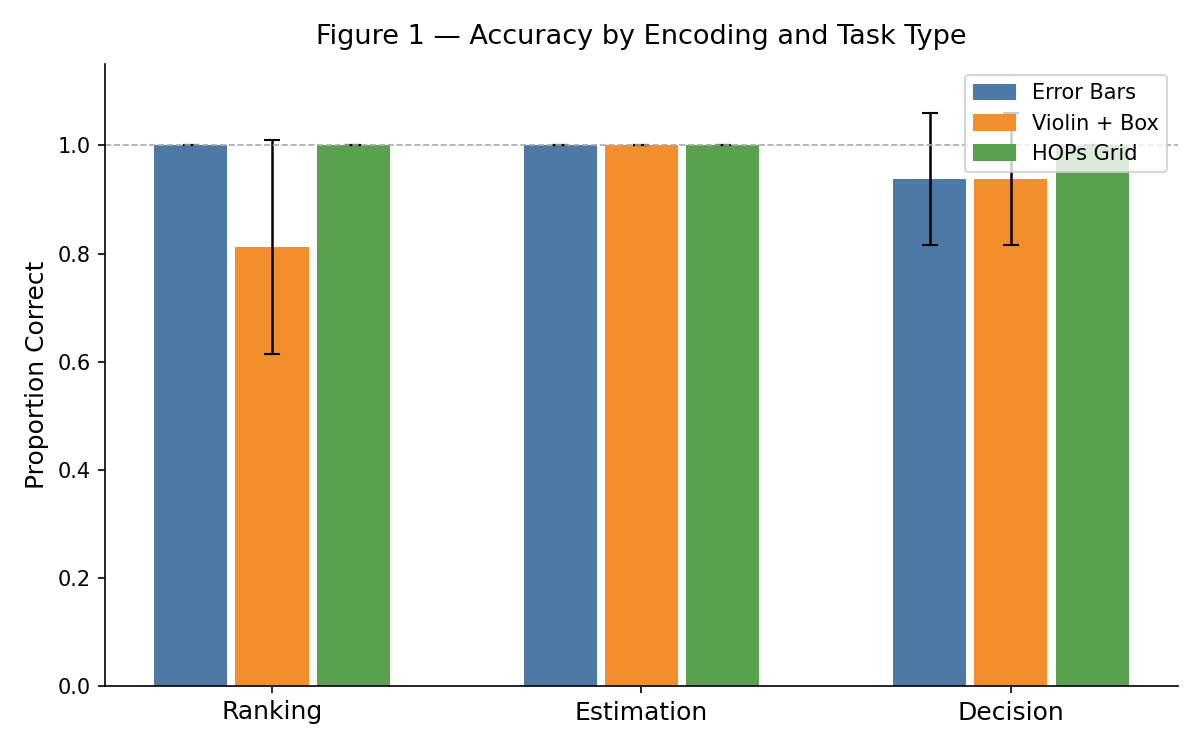
\includegraphics[width=\linewidth]{fig1_accuracy.png}
  \caption{Proportion correct by encoding and task type.  Error bars
    show 95\% confidence intervals.  Violin/box ranking is the only
    condition below ceiling.}
  \label{fig:accuracy}
\end{figure}

\subsection{Response Time}

Violin/box had the longest average response time (39.9\,s).  Error
bars (24.3\,s) and HOPs (26.1\,s) were comparable.  The Friedman test
on response time was not significant at $\alpha = 0.05$:
$\chi^2 = 4.63$, $df = 2$, $p = 0.099$, Kendall's $W = 0.145$
(a small effect).  Descriptively, violin/box was about $15.6$\,s
slower per trial than error bars and $13.8$\,s slower than HOPs, but
the within-participant pattern was inconsistent enough that the
omnibus test did not cross significance, and we did not run post-hoc
comparisons for that reason.  A larger sample might resolve this into
a significant effect, but we do not claim one here.

\begin{table}[ht]
\centering
\caption{Mean response time (seconds) by encoding and task type.}
\label{tab:time}
\rowcolors{2}{altrow}{white}
\begin{tabular}{lcccc}
\rowcolor{navyhead}
\color{white}\textbf{Encoding} &
\color{white}\textbf{Overall} &
\color{white}\textbf{Ranking} &
\color{white}\textbf{Estimation} &
\color{white}\textbf{Decision} \\
Error bars  & 24.3 & 23.8 & 25.9 & 23.2 \\
Violin/box  & 39.9 & 40.6 & 41.7 & 37.4 \\
HOPs grid   & 26.1 & 21.6 & 37.4 & 19.4 \\
\end{tabular}
\end{table}

Figure~\ref{fig:time} shows the distribution of response times by
encoding.  Violin/box had the widest spread and highest median, though
the Friedman test was not significant.

\begin{figure}[ht]
  \centering
  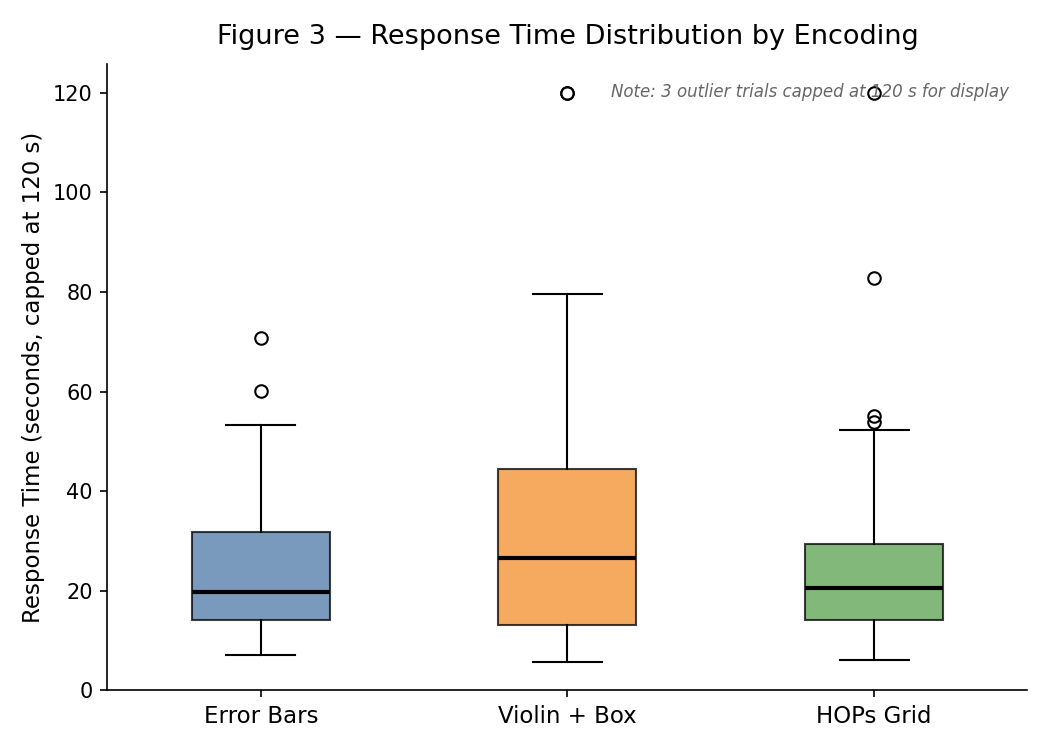
\includegraphics[width=\linewidth]{fig3_response_time.png}
  \caption{Response time distributions by encoding.  Boxes show the
    interquartile range; whiskers extend to 1.5$\times$IQR.}
  \label{fig:time}
\end{figure}

\subsection{Confidence and Calibration}

Mean confidence ratings were similar across encodings: error bars
(4.65/5), HOPs grid (4.50/5), and violin/box (4.42/5).  Brier scores
were low across the board, with error bars showing the best calibration
(0.025) and violin/box the worst (0.048).  The overconfidence index
was slightly \emph{negative} in every condition (error bars $-0.050$,
violin/box $-0.033$, HOPs $-0.100$), meaning participants were, if
anything, slightly underconfident relative to their near-perfect
accuracy.  This is the expected pattern when accuracy is pressed
against a 1.0 ceiling: stated confidence of $4/5$ ($= 0.8$) still
leaves a negative index when accuracy is $1.0$.  The narrow Brier
spread (0.025--0.048) should therefore be interpreted against this
ceiling, not as strong evidence that one encoding is meaningfully
better calibrated than another.

\begin{table}[ht]
\centering
\caption{Confidence and calibration by encoding.  The overconfidence
  index (OC) is mean confidence$/5$ minus mean accuracy; negative
  values indicate underconfidence.}
\label{tab:calibration}
\rowcolors{2}{altrow}{white}
\begin{tabular}{lccc}
\rowcolor{navyhead}
\color{white}\textbf{Encoding} &
\color{white}\textbf{Mean conf.\ (1--5)} &
\color{white}\textbf{Brier} &
\color{white}\textbf{OC index} \\
Error bars  & 4.65 & 0.025 & $-0.050$ \\
Violin/box  & 4.42 & 0.048 & $-0.033$ \\
HOPs grid   & 4.50 & 0.030 & $-0.100$ \\
\end{tabular}
\end{table}

Figure~\ref{fig:heatmap} provides a per-participant view of trial-level
correctness alongside each participant's age range and self-rated data
literacy.

\begin{figure}[ht]
  \centering
  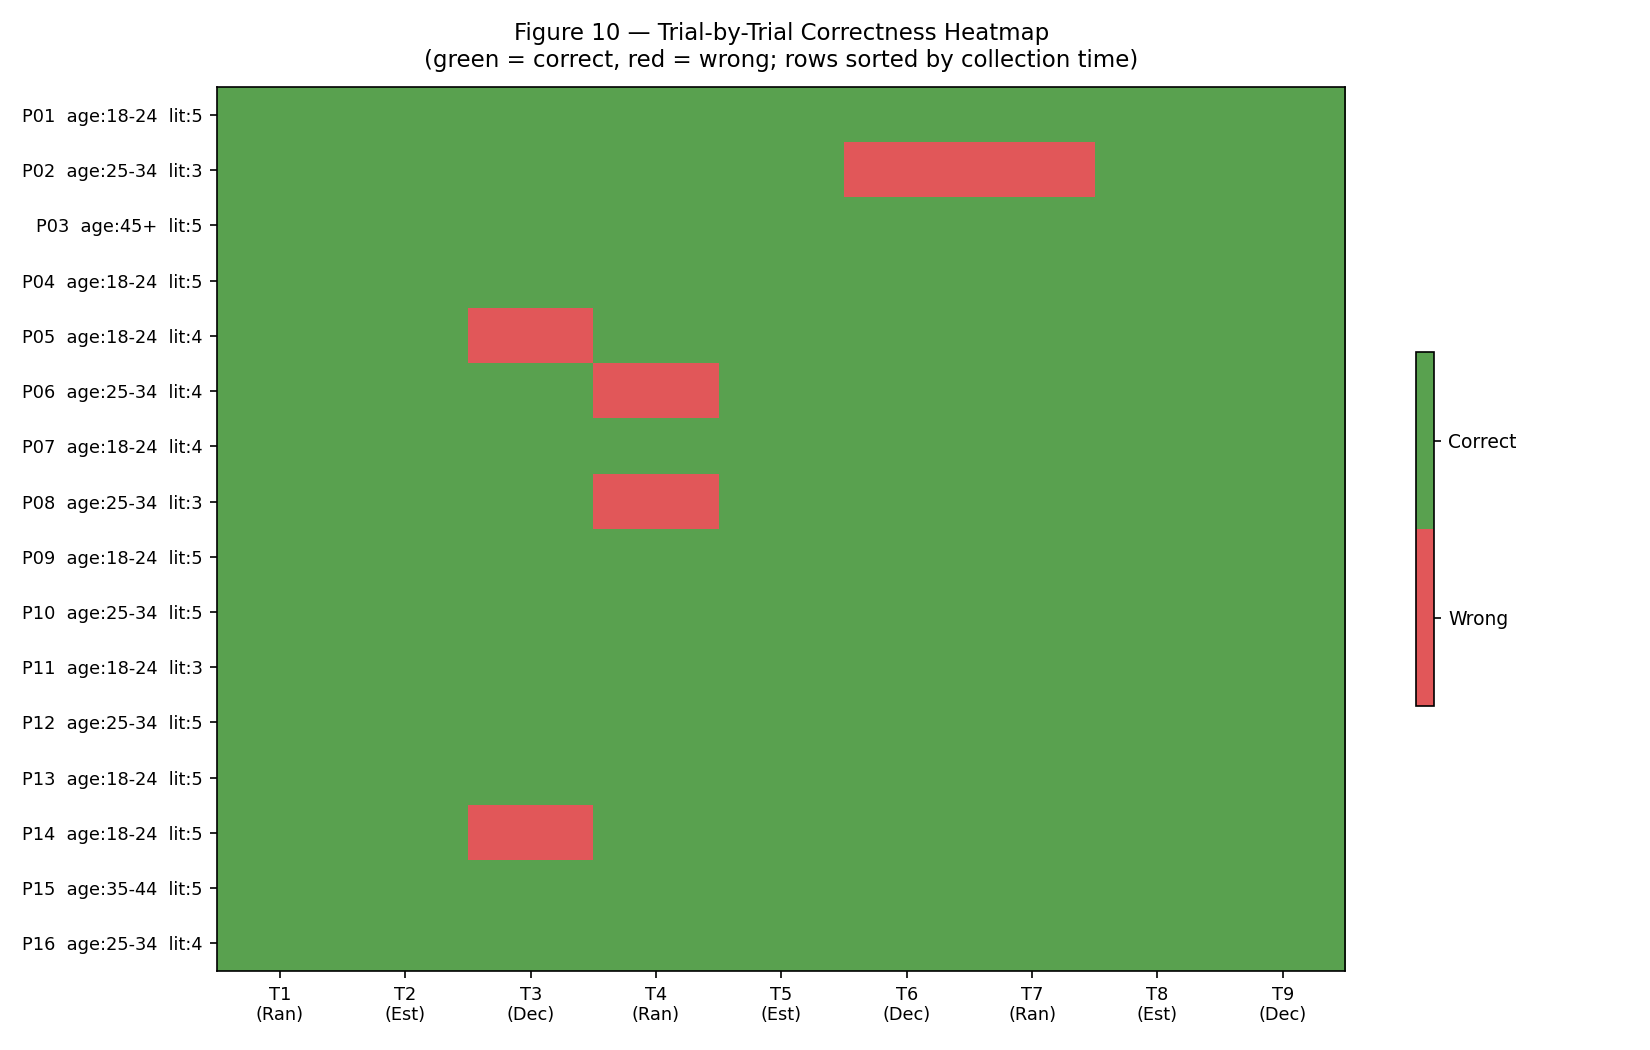
\includegraphics[width=\linewidth]{fig10_correctness_heatmap.png}
  \caption{Trial-level correctness heatmap for all 16 participants.
    Green cells indicate correct answers; red cells indicate errors.
    Age range and data literacy level are shown on the right axis.}
  \label{fig:heatmap}
\end{figure}

%======================================================================
\section{Discussion}
%======================================================================

\subsection{Interpretation of Results}

Our main-study accuracy pattern did not line up with H1 and H2 in the
way we expected: HOPs, not violin/box, led on accuracy, and violin/box
was actively worse than error bars on the ranking task.  A few
non-exclusive explanations are consistent with the data:

\begin{itemize}[leftmargin=*, itemsep=3pt]
\item \emph{Task-encoding alignment.}  Each HOPs panel makes the
  between-group ordering visible as a small picture; a participant
  doing a ranking task only has to scan panels and count
  ``which species is higher, most of the time.''  That is close to an
  optimal match between task and display.
\item \emph{Density dominance in violin/box.}  The violin's bulbous
  density silhouette is visually louder than the thin box-plot median
  line it wraps around.  On ranking, where the relevant cue is a
  single central tendency, the density shape seems to have pulled
  attention away from the median, leading the three outlier
  participants to rank by visual mass rather than by the embedded
  summary statistic.
\item \emph{Unfamiliarity as an attention cue.}  Participants had far
  more prior exposure to error bars than to HOPs, so the HOPs
  condition may have forced slower, more deliberate looking, while
  the familiar error bars may have encouraged a quicker pattern
  match.  Unfamiliarity can paradoxically improve accuracy on simple
  tasks by suppressing overlearned heuristics.
\item \emph{Cognitive load and ceiling effects.}  All three task
  types had a clear ground truth and a clean, well-separated dataset;
  the tasks were arguably too easy to discriminate the encodings,
  which is consistent with the high overall accuracy and the
  compressed Brier-score range.
\end{itemize}

Error bars had high accuracy (97.9\%) and the fastest response times
(24.3\,s), with the best numerical Brier score (0.025).  We are
cautious about calling them the best-calibrated encoding because, as
noted, the ceiling in accuracy mechanically compresses Brier score
across conditions; the ordering among 0.025, 0.030, and 0.048 is not
something we would bet on outside this specific task set.

\subsection{Calibration}

H2 (violin/box would produce the best calibration) was not supported.
Error bars had the numerically lowest Brier score, violin/box the
highest, and all three encodings sat in a narrow band where the
overconfidence index was slightly negative.  The most honest reading
is that accuracy near 1.0 mechanically caps how much Brier score can
vary between conditions.  A harder task set (for example a dataset
with more overlapping distributions, or with a noisy underlying
process) would be needed to test H2 on its own terms, because only
then would a participant who was genuinely \emph{over}confident be
able to show up in the data.

\subsection{Implications}

Read cautiously, these results suggest that for simple group-comparison
tasks on clean data, a static HOPs grid can match or slightly exceed
error bars on accuracy without imposing a clear additional time cost,
and that violin/box plots, despite being richer in information, may
actively mislead a subset of viewers on ranking tasks where the
density silhouette overwhelms the median.  None of those statements
is strong enough to act on without replication at a larger sample
size or with harder task sets, but the direction of the signal is
consistent with earlier HOPs work~\cite{hullman2015} even though our
HOPs were static rather than animated.

\subsection{Limitations}

\begin{itemize}[leftmargin=*, itemsep=4pt]
\item \emph{Ceiling effects.}  Accuracy was at or near $100\%$ in
  every encoding, which mechanically compresses differences on both
  accuracy and Brier score and limits what the omnibus test can see.
\item \emph{Small sample.}  $n = 16$ is small for Friedman-style
  tests; effect-size estimates are unstable and the significant
  omnibus result on accuracy did not survive Bonferroni correction in
  the post-hoc pairwise tests.  We should treat this as pilot-scale
  evidence.
\item \emph{Sample composition.}  The convenience sample was
  recruited from a Bay Area / Silicon Valley peninsula social network
  with an above-average density of current and former STEM graduate
  students and industry engineers.  Self-rated data literacy was
  correspondingly high (median $= 5/5$).  This biases performance
  upward in every condition and is likely part of why the data hit
  ceiling; a sample drawn from the general public would almost
  certainly show lower absolute accuracy and, possibly, wider spreads
  between encodings.
\item \emph{Task simplicity.}  Three task types on a clean,
  well-separated dataset with three well-known species.  The Adelie
  mean in particular is so far from the other two that most
  participants likely did not need any uncertainty information to
  answer ranking and decision questions correctly.
\item \emph{Static HOPs only.}  Animated HOPs, which is the original
  form in \cite{hullman2015}, were not tested.  The static grid is a
  practical simplification, not a faithful replication of prior
  HOPs work.
\item \emph{Parallel task sets.}  Parallel sets reduced answer
  carry-over but introduced slight content variation between blocks
  (different ranking targets, different estimation species).  Any
  leftover difficulty asymmetry between sets could show up as
  encoding difference because of the within-subjects block
  assignment.
\item \emph{Environmental inconsistency.}  Most sessions were
  proctored over Zoom or FaceTime, but a few participants used the
  hosted link independently.  Proctor presence can introduce
  implicit time pressure, compress reading, and change the set of
  clarifying questions participants ask.  This adds noise to the
  response-time measure in particular.
\end{itemize}

\subsection{Suggestions for Future Research}

\begin{itemize}[leftmargin=*, itemsep=4pt]
\item Test animated HOPs against the same baselines to see if motion
  further improves the advantage seen with the static grid.
\item Use more complex tasks (trend detection, outlier identification)
  where distributional shape should matter more.
\item Recruit a larger and more diverse sample, including domain
  scientists outside of STEM computing fields.
\item Test on noisier datasets where group differences are less
  obvious.
\item Explore hybrid encodings that combine error bars with
  distributional overlays.
\end{itemize}

%======================================================================
\section{Conclusion}
%======================================================================

On common group-comparison tasks over a clean, well-separated dataset,
a static HOPs grid slightly outperformed both error bars and
violin/box plots on accuracy, while error bars were numerically the
fastest and best-calibrated encoding.  Violin/box carried a
descriptive cost on the ranking task and on per-trial response time,
though neither cost was large enough to survive the conservative
statistical thresholds once sample size and ceiling effects were
taken into account.

We present these results as pilot-scale, directional evidence rather
than as a definitive recommendation.  They are consistent with the
broader finding in the HOPs literature~\cite{hullman2015} that
showing multiple plausible outcomes can help viewers reason about
uncertainty, and they suggest a concrete follow-up: the same design
with a harder stimulus set (more overlapping distributions, noisier
data), a larger and more diverse sample, and an animated HOPs
condition to pair against the static grid.

The study's primary contribution is methodological: a controlled,
within-subjects comparison of three widely used general-purpose
uncertainty encodings on three standardized task types, with explicit
definitions of \emph{correct}, an overconfidence index alongside the
Brier score, and a participant-level, tie-corrected non-parametric
analysis.  That combination fills a gap in the recent literature,
which has focused on formal frameworks, modality comparisons, or
domain-specific solutions rather than on head-to-head empirical tests
of the general-purpose encodings that most practitioners actually
reach for.

\subsection*{Closing Thoughts}

Uncertainty communication sits at the intersection of statistics,
perception, and design, and most scientific figures still default to
a simple error bar.  Even at this pilot scale, the data suggest the
default is not automatically the best choice, and that encoding
decisions are empirical questions as much as aesthetic ones.  Scaled
up to harder tasks and a more diverse sample, this line of work
could produce practical guidance that meaningfully improves how
uncertainty reaches the readers of scientific figures.

\section*{Acknowledgments}

Thanks to the participants who volunteered their time, and to
Professor Shelley Wong for advising on study design and providing feedback
throughout the project.

\printbibliography

\end{document}
